\documentclass[11pt]{article}

\usepackage[french]{babel}
\usepackage[utf8x]{inputenc}  
\usepackage[T1]{fontenc}
\usepackage[left=2.7cm,right=2.7cm,top=3cm,bottom=3cm]{geometry}
\usepackage{amsmath,amssymb,amsfonts}
\usepackage{kpfonts}
\usepackage{tikz}
\usepackage{bbm}
\usepackage{hyperref}
\usepackage{algorithm}
\usepackage{algpseudocode}

\graphicspath{{ims/}}

\newcommand{\trans}{\mathsf{T}}
\newcommand{\syst}[2]{\left\{ \begin{array}{#1} #2 \end{array} \right.}
\newcommand{\pmat}[1]{\begin{pmatrix} #1 \end{pmatrix}}
\newcommand{\R}{\mathbb{R}}
\newcommand{\N}{\mathbb{N}}

\DeclareMathOperator{\trace}{tr}
\DeclareMathOperator{\grad}{grad}
\DeclareMathOperator{\divergence}{div}
\DeclareMathOperator{\connexionLaplacian}{\Delta^{\hspace{-3pt} \nabla}}
\DeclareMathOperator*{\argmin}{arg\,min}


\title{
	\noindent\rule{\linewidth}{0.4pt}
	{ \huge Modèles Déformables et Méthodes Géodésiques en Analyse d’images } \\
	Projet : The Vector Heat Method \cite{VHM}
	\noindent\rule{\linewidth}{1pt}
}
\date{31 mai 2020}

\author{Yoann Coudert-\,-Osmont}

\begin{document}
	
	\maketitle
	
	\section{Etude synthétique de l'article}
	
	\paragraph{Problème traité}
	Le papier propose une méthode pour transporter parallèlement un vecteur suivant les géodésiques d'une variété. Cette méthode donne par la suite, la possibilité de calculer le $\log$ riemannien de manière efficace, de calculer des moyennes de Fréchet, de construire des tesselations de Voronoï centrées, ou encore de calculer des \textit{landmarks} ordonnés.
	
	\paragraph{Equations et méthodes numériques utilisées}
	L'équation de la chaleur est utilisée pour calculer les distances géodésiques. Comme on a pu le voir en TP, cette méthode est très efficace et converge sous certaines conditions vers les vrais distances géodésiques. Ainsi les géodésiques ne sont pas calculées explicitement. Ces calculs généralement complexes sont remplacés par de simples résolutions de systèmes linéaires creux. Ces systèmes sont définis avec un Laplacien qui est défini sur beaucoup de types de données différentes (maillages polygonaux, nuages de points, surfaces splines, voxels ...) ce qui en fait un point fort de ce papier, l'adaptabilité. En revanche le papier commence par donner une définition formelle d'un Laplacien applicable à des champs de vecteurs (appelé Laplacien de connexion), mais par la suite la construction de la discrétisation de cet opérateur est décrite et justifiée par l'intuition sans faire de lien direct avec la définition mathématique donnée initialement. C'est dommage, une justification mathématique aurait pu être appréciable.
	
	\paragraph{Comparaison avec le cours}
	On retrouve l'équation de la chaleur que nous avons utilisé dans un TP pour calculer des distances géodésiques et pour échantillonner un maillage à faces triangulaires. Ce papier publié à SIGGRAPH, se veut plus orienté graphismes et géométrie algorithmique et en ce sens s'éloigne plus du cours que les autres papiers proposés en projet. Toutefois, la première application donnée dans le papier est complètement en lien avec le cours puisqu'ils proposent d'utiliser le transport parallèle pour extrapoler la composante normale de la vitesse dans la méthode des courbe de niveau sur une variété. De plus la dernière application proposée est un calcul de \textit{landmarks} intrinsèques ordonnés sur une géométrie qui utilise un échantillonnage de points les plus éloignés. On a pu voir en cours un tel échantillonnage en utilisant l'algorithme \textit{fast marching} ou même en TP en utilisant la diffusion de la chaleur.
	
	\paragraph{Originalité (selon les auteurs)}
	Ce papier est dans la continuité d'un précédent papier de Keenan Crane, sur le calcul des distances géodésiques via l'équation de la chaleur \cite{HM}. Leur approche est original dans le sens où ils semblent être les seuls à avoir creusé cette approche par l'équation de la chaleur pour le transport parallèle. Les approches précédentes se basaient généralement sur un calcul explicite des géodésiques. Or calculer toutes les distances à partir d'un sommet de manière exacte a une complexité en $\mathcal{O}(n^2 \log n)$, où $n$ est le nombre d'arrêtes. Cette complexité est bien trop grande et les algorithmes qui approximent ces géodésiques à moindre coût peuvent donner des résultats trop différents et ont une complexité au minimum de l'ordre de $\mathcal{O}(n^{1.5})$ puisque la longueur d'une géodésique est de l'ordre de $\mathcal{O}(\sqrt{n})$. Ici la solution proposé possède une complexité proche de $\mathcal{O}(n)$ et les résultats sont très satisfaisant. Je n'ai testé, mais les auteurs précisent que le simple fait de tracer les géodésiques est 10 à 20 fois plus long que leur méthode de transport parallèle.
	
	\paragraph{Résultats nouveaux}
	Selon eux, les auteurs seraient les premiers à proposé un calcul de la carte logarithme efficace. Les anciennes méthodes ne calculaient le logarithme que dans un voisinage de la source (et extrapolaient éventuellement au reste). Selon une figure donnée dans l'article les anciennes méthodes engendraient des erreurs non négligeables sur l'orientation pour les sommets assez éloignés du sommet initial, alors que la méthode présentée dans ce papier donne de très bon résultats. De plus ce calcul efficace du $\log$ entraîne immédiatement une première méthode de calcul de moyennes de Fréchet précise et efficace. Encore une fois, les comparaisons faites avec les précédentes méthodes sont assez bluffantes et le temps de calcul bien moindre.
	
	\paragraph{Faiblesses}
	La méthode possède tout de même des défauts. En effet l'orientation des vecteurs a tendance à être mauvaise au niveau des lignes de coupures (l'ensemble des sommets qui possèdent plusieurs plus courts chemin vers la source, voir \figurename~\ref{fig:cut_locus}). De plus les résultats dépendent énormément de la qualité du maillage (plus les triangles sont proches d'un triangle équilatéral meilleur est la qualité, voir \figurename~\ref{fig:car}). Mais la solution proposée consistant à effectuer au préalable une triangulation de Delaunay semble être un bon remède. On remarque aussi que dans le cas de sources multiples, certaines propriétés du transport optimal sont perdus. Enfin dans le cas du calcul des distances géodésiques via l'équation de la chaleur, Keenan Crane et ses collègues avaient réussi à formuler de bonnes conditions aux bords dans le cas de surfaces à bords (une moyenne entre les conditions de Dirichlet et de Neumann était faite). Mais ici rien de tel n'est proposé. Je n'ai pas implémenté les conditions au bord de Dirichlet mais les auteurs ont l'air de dire que les résultats sont similaires aux conditions de Neumann. Il pourrait être bien de creuser pour améliorer ces conditions.
	
	\section{Résumé}
	
	\subsection{Source unique}
	Pour un champs scalaire $\phi_t$ qui évolue au cours du temps on rappelle que l'équation de la chaleur s'écrit :
	$$ \frac{d}{dt} \phi_t = \Delta \phi_t $$
	Où $\Delta$ est l'opérateur Laplacien défini comme la divergence du gradient ou encore, comme la trace de la Hessienne :
	$$ \Delta f = \trace \left( H(f) \right) = \divergence \circ \grad f $$
	Pour un champ de vecteur on peut définir une équation de la chaleur de manière similaire. On remplace simplement le gradient par une dérivée covariante/connexion. Et on remplace les opérateurs qui découlent directement du gradient par les opérateurs qui découlent directement d'une connexion. Le papier propose naturellement la connexion de Levi-Civita $\nabla$. On peut alors définir un Laplacien de connexion $\connexionLaplacian$ par :
	$$ \connexionLaplacian X = \trace \left( \nabla^2 X \right) = - \nabla^* \nabla X $$
	Où la dérivée covariante seconde est définie comme suit :
	$$ \nabla^2_{X, Y} Z = \nabla_X \nabla_Y Z - \nabla_{\nabla_X Y} Z $$
	Et où $\nabla^*$ est l'adjoint de la connexion.
	En prenant pour champs de vecteur au temps zéro, $X_0 = \delta_x v$ le champs valant $v$ en $x$ et nul partout ailleurs, la solution de l'équation de la chaleur vectorielle s'écrit alors :
	$$ k_t^\nabla(x, y) \cdot v = \frac{e^{-d(x, y)^2 / 4t}}{(4 \pi t)^{n/2}} j(x, y)^{-1/2} \left( \sum_{i=0}^\infty t^i \Psi_i(x, y) \right) \cdot v $$
	Où la première fonction de la série est l'opérateur de transport parallèle le long de la géodésique minimale entre $x$ et $y$ :
	$$ \Psi_0(x, y) = P_{\gamma_{x \rightarrow y}} $$
	En ce sens, lorsque $t$ tend vers 0, la solution se trouve être le transport parallèle de $v$ selon les géodésiques à une constante multiplicative près variant selon la position $y$. Cette constante multiplicative est la solution de l'équation de la chaleur scalaire partant d'un champs initial $\phi_0 = \delta_x |v|$ valant la norme de $v$ en $x$ et étant nul partout ailleurs. On note cette solution $k_t(x, y)$, et on obtient :
	$$ \lim_{t \rightarrow 0} \frac{k_t^\nabla(x, y)}{k_t(x, y)} = P_{\gamma_{x \rightarrow y}} $$
	
	\subsection{Multiples sources}
	
	Dans le cas où notre champ initial n'est plus un simple Dirac mais un champ sur une partie $\Omega \subset M$ de notre variété, on souhaite que le vecteur obtenu au point $q$ soit le transporté du vecteur au point $p$ de $\Omega$ le plus proche. On note alors $X$ le champs de vecteur initial nul sur $M \setminus \Omega$, et $\bar{X}$ le champ obtenu par transport parallèle. On utilisera la notation $X|_p$ pour la valeur du champ $X$ au point $p$. On souhaite obtenir le champ suivant :
	$$ \bar{X}|_q = \syst{ll}{
		X|_q & \text{Si } q \in \Omega \\
		P_{\gamma_{p \rightarrow q}} \cdot X|_p & \text{Si } q \notin \Omega \text{ et } p = \argmin_{r \in \Omega} d(q, r)
	} $$
	Soit alors deux scalaires distincts $u$ et $v$ et deux positions $x$ et $y$ sur $M$. On remarque la limite suivante :
	$$ \lim_{t \rightarrow 0} \frac{u k_t(x, z) + v k_t(y, z)}{k_t(x, z) + k_t(y, z)} = \syst{ll}{
		u & \text{Si } d(x, z) < d(y, z) \\
		v & \text{Si } d(x, z) > d(y, z) \\
		(u+v) / 2 & \text{Si } d(x, z) = d(y, z) \\
	} $$
	Le numérateur est la solution de la diffusion de $\delta_x u + \delta_y v$ alors que le dénominateur est la solution de $\delta_x + \delta_y$. La fraction constituée retourne ainsi la valeur associée au point le plus proche (voir \figurename~\ref{fig:voronoi}). On peut étendre cette idée à un domaine $\Omega$ quelconque afin de renormaliser correctement notre champ vectorielle après diffusion. Il suffit alors de considéré les solutions des équations suivantes :
	$$ \frac{d}{dt} u_t = \Delta u_t \qquad \text{avec } \quad u_0 = | X | $$
	$$ \frac{d}{dt} \phi_t = \Delta \phi_t \qquad \text{avec } \quad \phi_0 = \mathbbm{1}_\Omega $$
	Puis on définira la norme de $\bar{X}$ via :
	$$ | \bar{X} | = u_t / \phi_t $$
	La direction de $\bar{X}$ en revanche sera celle obtenue via la résolution de l'équation de la chaleur au temps $t$ partant de la condition initiale $\bar{X}_0 = X$. Cela permet alors de définir l'algorithme \ref{alg:VHM} pour calculer le transport parallèle d'un champ de vecteur. Un exemple est donné \figurename~\ref{fig:parallel}.
	
	\begin{figure}
		\centering
		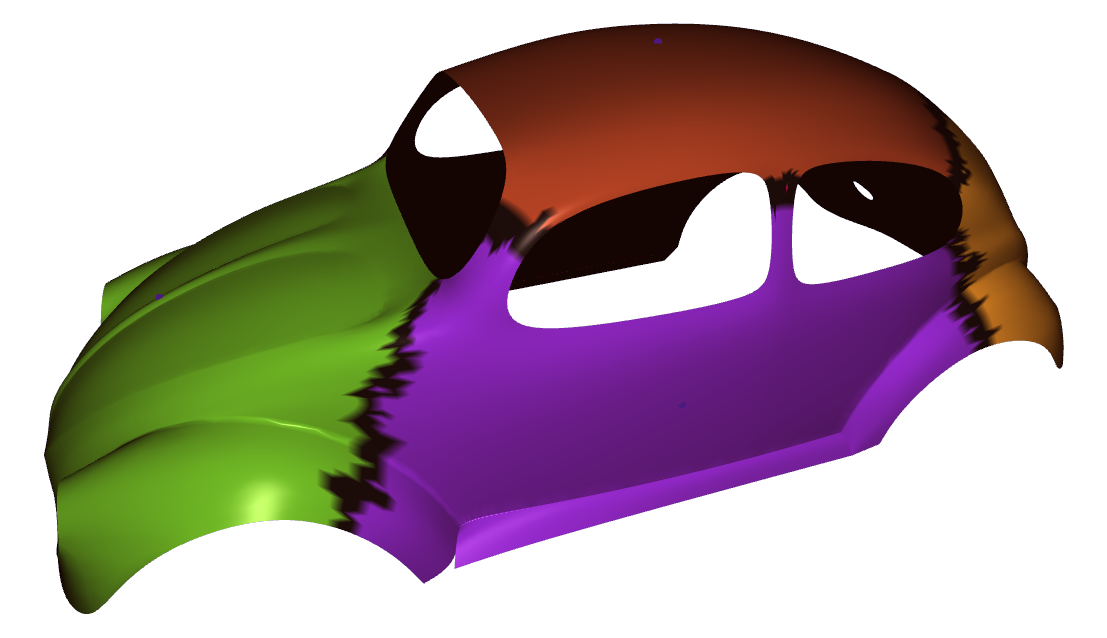
\includegraphics[width=12cm]{voronoi_car.png}
		\caption{Champ scalaire $u_t / \phi_t$ obtenu à partir de plusieurs sources sur la maillage \texttt{beetle.off}. Un entier $u_t|_i$ et une couleur ont été associés à chaque source $i$. Le résultat obtenu est bien une interpolation par plus proche voisin.}
		\label{fig:voronoi}
	\end{figure}
	
	\begin{algorithm}[h]
		\caption{Vector Heat Method}
		\label{alg:VHM}
		\begin{algorithmic}
			\State \textbf{Entrée:} Un champ de vecteur $X$ sur une partie $\Omega$ d'une variété $M$.
			\State \textbf{Sortie:} Un champ de vecteur $\bar{X}$ sur $M$ tout entier.
			\State \hspace{10pt} I. \; Résoudre $\frac{d}{dt} Y_t = \connexionLaplacian Y_t$ au temps $t$ avec la condition initiale $Y_0 = X$.
			\State \hspace{6pt} II. \; Résoudre $\frac{d}{dt} u_t = \Delta u_t$ au temps $t$ avec la condition initiale $u_0 = |X|$.
			\State \, III. \; Résoudre $\frac{d}{dt} \phi_t = \Delta \phi_t$ au temps $t$ avec la condition initiale $\phi_0 = \mathbbm{1}_\Omega$.
			\State \hspace{3pt} IV. \; Construire le champ de vecteur $\bar{X}_t = ( u_t Y_t) / (\phi_t |Y_t|)$.
		\end{algorithmic}
	\end{algorithm}

	\subsection{Discrétisation}
	
	Bien que la méthode présentée soit très générale, le papier propose une discrétisation dans le cas de champs de vecteurs sur des maillages triangulaires. Il y est suggéré de représenter un vecteur $v$ tangent au maillage en un sommet $i$ par un complexe $z$ dont le module encode la norme de $v$, et l'argument, son angle $\varphi_{iv}$ avec le vecteur $\overrightarrow{ij_0}$ où $j_0$ est un voisin de $i$ choisi arbitrairement.
	\begin{center}
		\begin{tikzpicture}[scale=1.3]
			\coordinate (i) at (0, 0);
			\coordinate (j0) at ({1.3*cos(44)}, {-1.3*sin(44)});
			\coordinate (j1) at (1.5, 0);
			\coordinate (j2) at (0.9, 1);
			\coordinate (j3) at (-0.8, 1);
			\coordinate (j4) at (-1.4, 0.1);
			\coordinate (j5) at (-0.9, -0.9);
			
			\draw[thick] (i) -- (j0) -- (j1) -- (i) -- (j2) -- (j3) -- (i) -- (j4) -- (j5) -- (i);
			\draw[thick] (j1) -- (j2);
			\draw[thick] (j3) -- (j4);
			\draw[thick] (j5) -- (j0);
			
			\node[above] at (i) {$i$};
			\node[below] at (j0) {$j_0$};
			\draw[->, thick, red] (i) -- ({1.2*cos(30)}, {1.2*sin(30)}) node[below=1pt] {$v$};
			\node at (i) {$\bullet$};
			\node at (j0) {$\bullet$};
			\node at (j1) {$\bullet$};
			\node at (j2) {$\bullet$};
			\node at (j3) {$\bullet$};
			\node at (j4) {$\bullet$};
			\node at (j5) {$\bullet$};
			\node[blue, right] at (1.3, 0.6) {$z = |v| e^{\iota \varphi_{iv}}$};
			\draw[thick, blue] ({0.45*cos(44)}, {-0.45*sin(44)}) arc(-44:30:0.45) node[pos=0.3, right] {$\varphi_{iv}$};
		\end{tikzpicture}
	\end{center}
	
	Les détails pour définir l'angle $\varphi$ sont donnés dans le papier, mais je ne les redonnerai pas, car ce n'est pas d'une importance capitale. On note par la suite $\varphi_{ij}$ l'angle entre les vecteurs $\overrightarrow{ij_0}$ et $\overrightarrow{ij}$ pour $j$ un voisin de $i$. Ainsi le vecteur $\overrightarrow{ij}$ est représenté par l'angle $\varphi_{ij}$ dans la face $i$ et par l'angle $\varphi_{ji} + \pi$ dans la face $j$. Pour représenter un vecteur un vecteur de la face $j$ dans la face $i$ il suffit alors de multiplier par le complexe :
	$$ r_{ij} = \exp \left( \iota \left( \varphi_{ij} - \varphi_{ji} + \pi \right) \right) $$
	\begin{center}
		\begin{tikzpicture}[scale=1.3]
			\coordinate (i) at (0, 0);
			\coordinate (j0) at ({1.3*cos(44)}, {-1.3*sin(44)});
			\coordinate (j1) at (1.5, 0);
			\coordinate (j2) at (0.9, 1);
			\coordinate (j3) at (-0.8, 1);
			\coordinate (j4) at (-1.4, 0.1);
			\coordinate (j5) at (-0.9, -0.9);
			\coordinate (j6) at (2.3, -1);
			\coordinate (j7) at (2.9, -0.1);
			\coordinate (j8) at ({1.5+1.2*cos(50)}, {1.2*sin(50)});
			
			\draw[thick] (i) -- (j0) -- (j1) -- (j2) -- (i) -- (j3) -- (j4) -- (i) -- (j5) -- (j0) -- (j6) -- (j1) -- (j7) -- (j8) -- (j2);
			\draw[very thick, red] (i) -- (j1);
			\draw[thick] (j2) -- (j3);
			\draw[thick] (j4) -- (j5);
			\draw[thick] (j8) -- (j1);
			\draw[thick] (j6) -- (j7);
			
			\node[above] at (i) {$i$};
			\node[below] at (j0) {$j_0$};
			\node at (i) {$\bullet$};
			\node at (j0) {$\bullet$};
			\node at (j1) {$\bullet$};
			\node[below] at (j1) {$j$};
			\node at (j2) {$\bullet$};
			\node at (j3) {$\bullet$};
			\node at (j4) {$\bullet$};
			\node at (j5) {$\bullet$};
			\node at (j6) {$\bullet$};
			\node at (j7) {$\bullet$};
			\node at (j8) {$\bullet$};
			\node[right] at (j8) {$k_0$};
			\draw[thick, blue] ({0.45*cos(44)}, {-0.45*sin(44)}) arc(-44:0:0.45) node[pos=0.3, right] {$\varphi_{ij}$};
			\draw[thick, blue] ({1.5+0.3*cos(50)}, {0.3*sin(50)}) arc(44:180:0.3) node[pos=0.3, above=-2pt] {$\varphi_{ji}$};
		\end{tikzpicture}
	\end{center}
	Ainsi en reprenant le Laplacien cotangent $L$ pour un maillage triangulaire (vu en TP), on peut définir le Laplacien de connexion $L^\nabla$ via :
	$$ L_{ij}^\nabla = \syst{ll}{
		L_{ij} & \text{Si } i = j \\
		r_{ij} L_{ij} & \text{Si } i \neq j
	} $$
	Comme $r_{ji} = \overline{r_{ij}}$, la matrice $L^\nabla$ construite est Hermitienne en supposant que $L$ soit symétrique.
	
	\begin{figure}
		\centering
		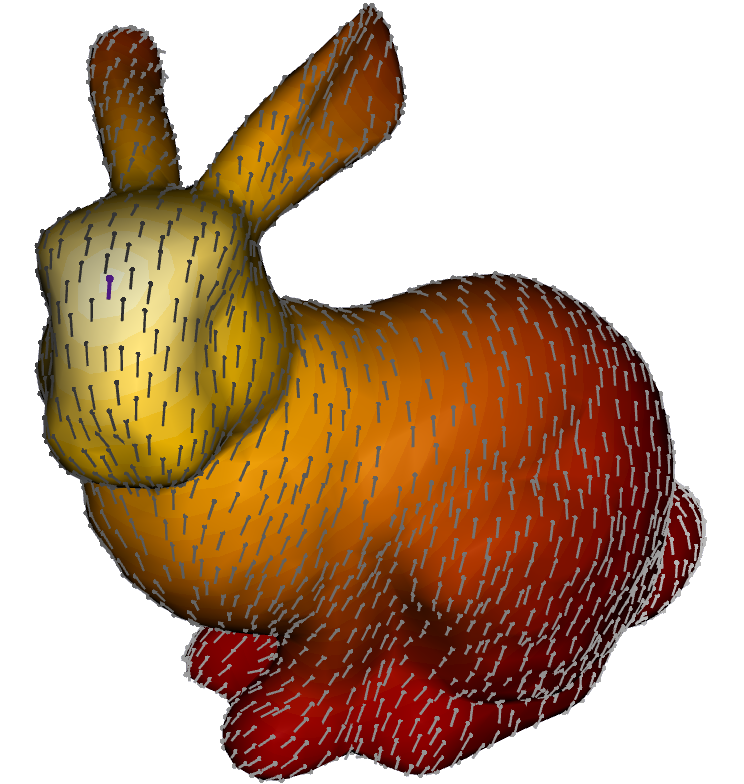
\includegraphics[width=8.5cm]{parallel_transport.png}
		\caption{Transport parallèle d'une source unique au milieu de la tête du lapin (représenté par un vecteur bleu/violet).}
		\label{fig:parallel}
	\end{figure}
	
	
	\paragraph{Triangulation intrinsèque de Delaunay}
	Enfin la qualité du maillage a son importance sur le résultat (ex : \figurename~\ref{fig:orientation_delaunay}). Dans le cas de sources multiples, les vecteurs à équidistances de deux sources peuvent avoir des orientations voir des normes erronés (ex : \figurename~\ref{fig:norme_delaunay}). Pour palier à cela, les auteurs du papier proposent d'effectuer une triangulation intrinsèque de Delaunay comme cela a déjà été proposé avant pour le calcul des distances géodésiques via la propagation de la chaleur.
	
	
	\begin{figure}
		\centering
		\begin{tikzpicture}
		\node at (0,0) {\fbox{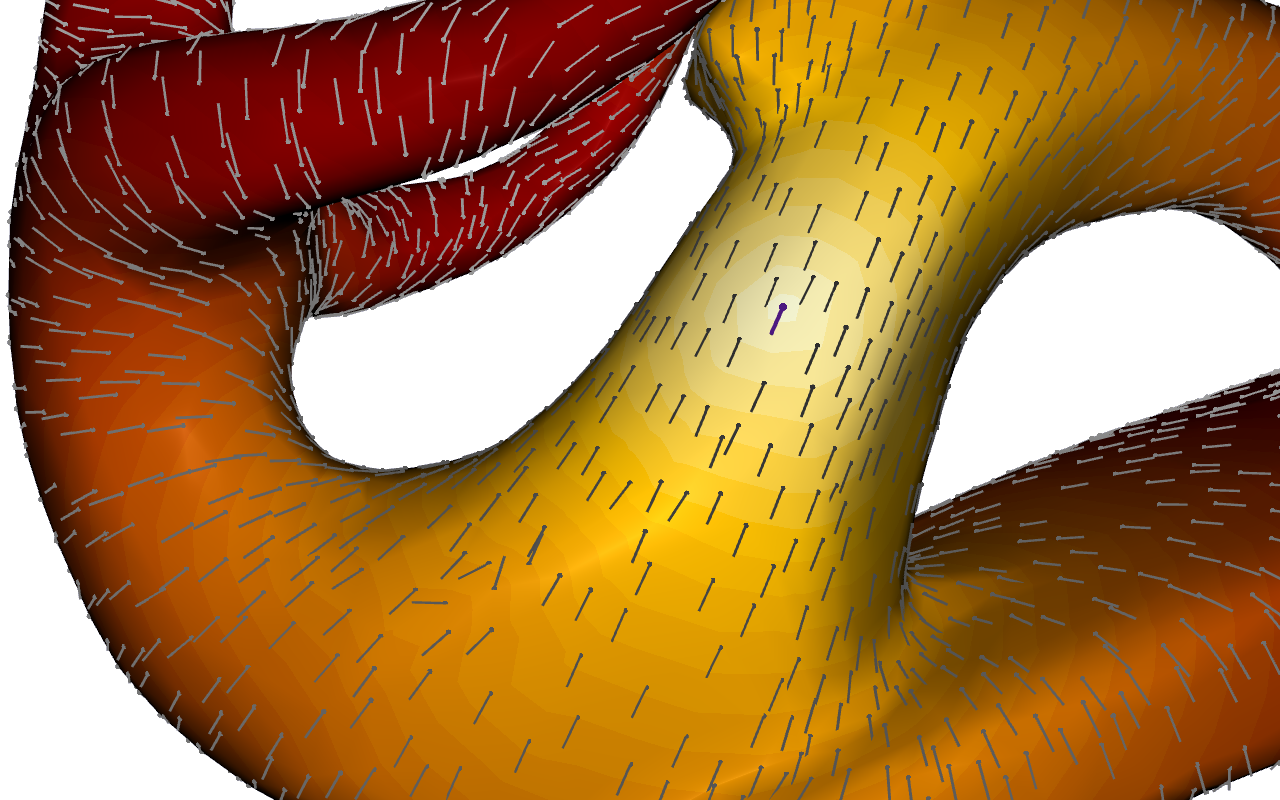
\includegraphics[width=7.5cm]{without_delaunay.png}}};
		\draw[blue, thick] (-1.1, -1.02) circle(1.22);
		\node at (8,0) {\fbox{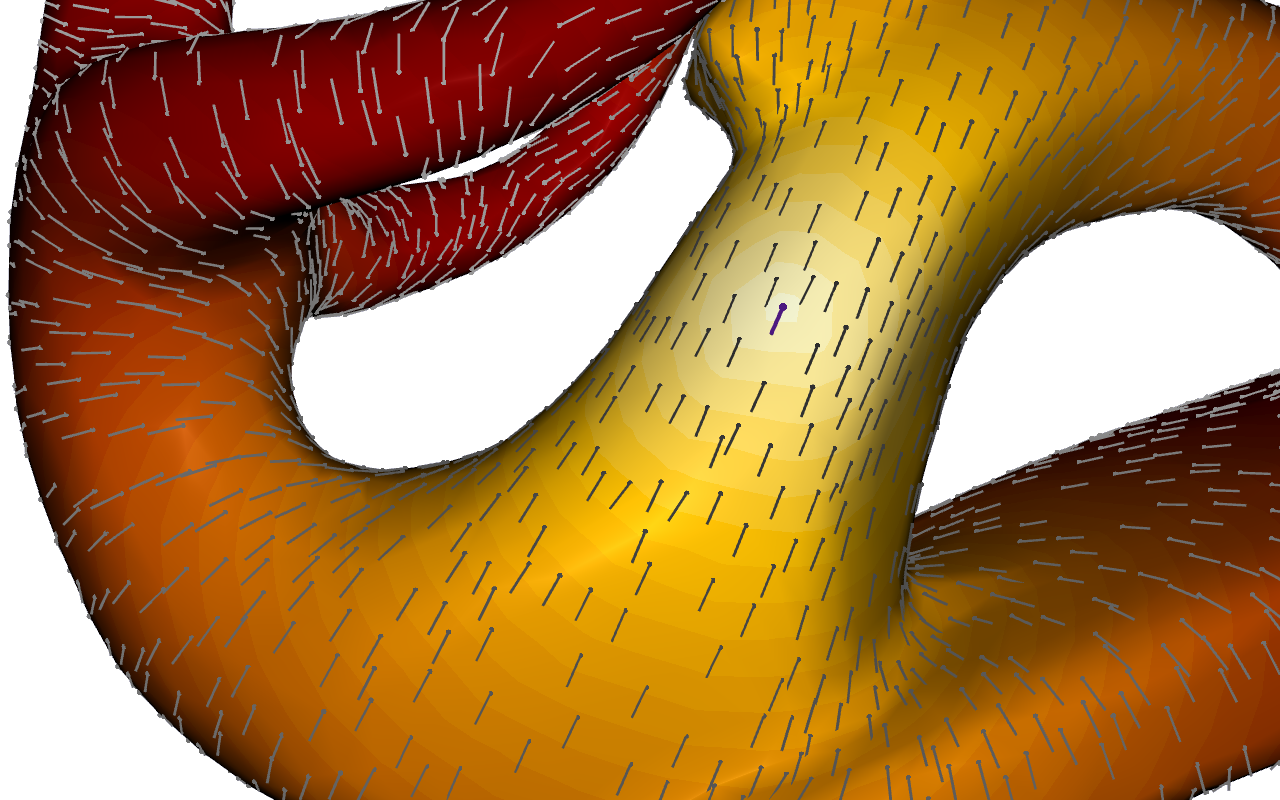
\includegraphics[width=7.5cm]{with_delaunay.png}}};
		\draw[blue, thick] (6.9, -1.02) circle(1.22);
		\end{tikzpicture}
		\vspace{-5pt}
		\caption{Champs de vecteurs obtenus par transport optimal d'une source unique. A gauche la triangulation du maillage a été utilisée, à droite on utilise la triangulation de Delaunay. On remarque des défauts dans l'image de gauche qu'on ne retrouve pas à droite.}
		\label{fig:orientation_delaunay}
	\end{figure}

	\begin{figure}
		\centering
		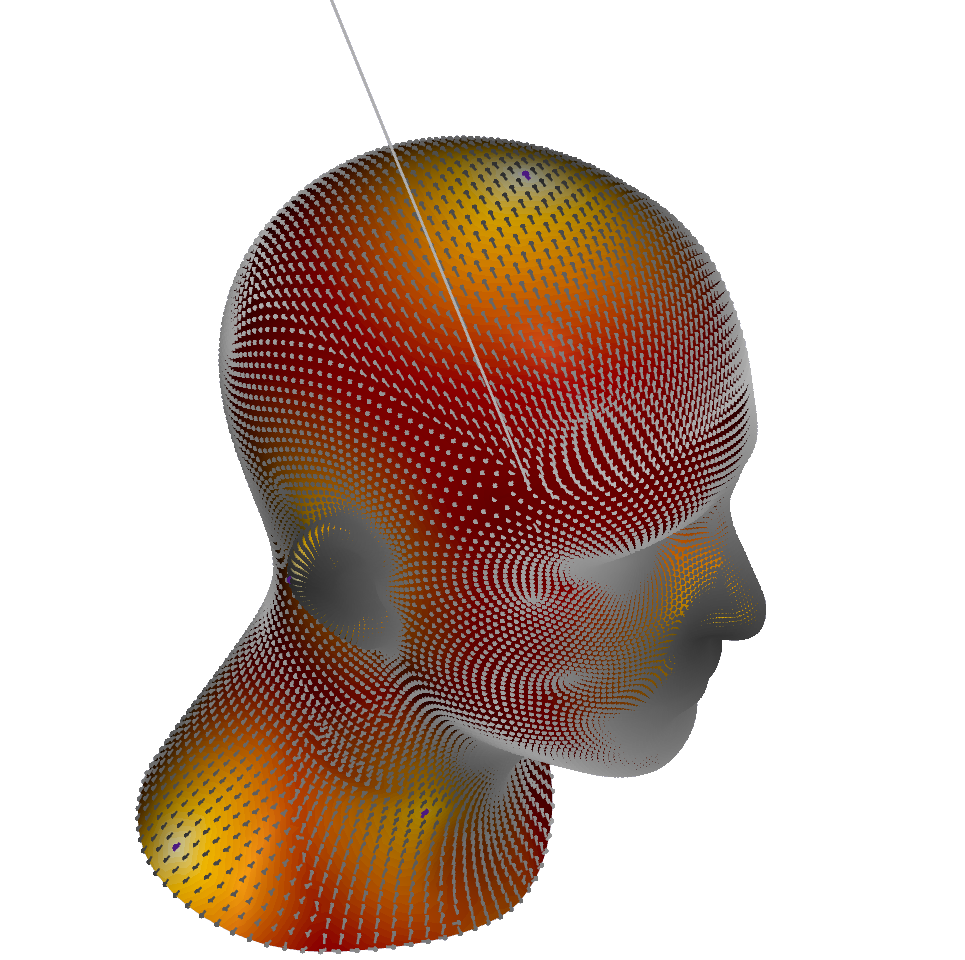
\includegraphics[width=7cm]{face.png} \; 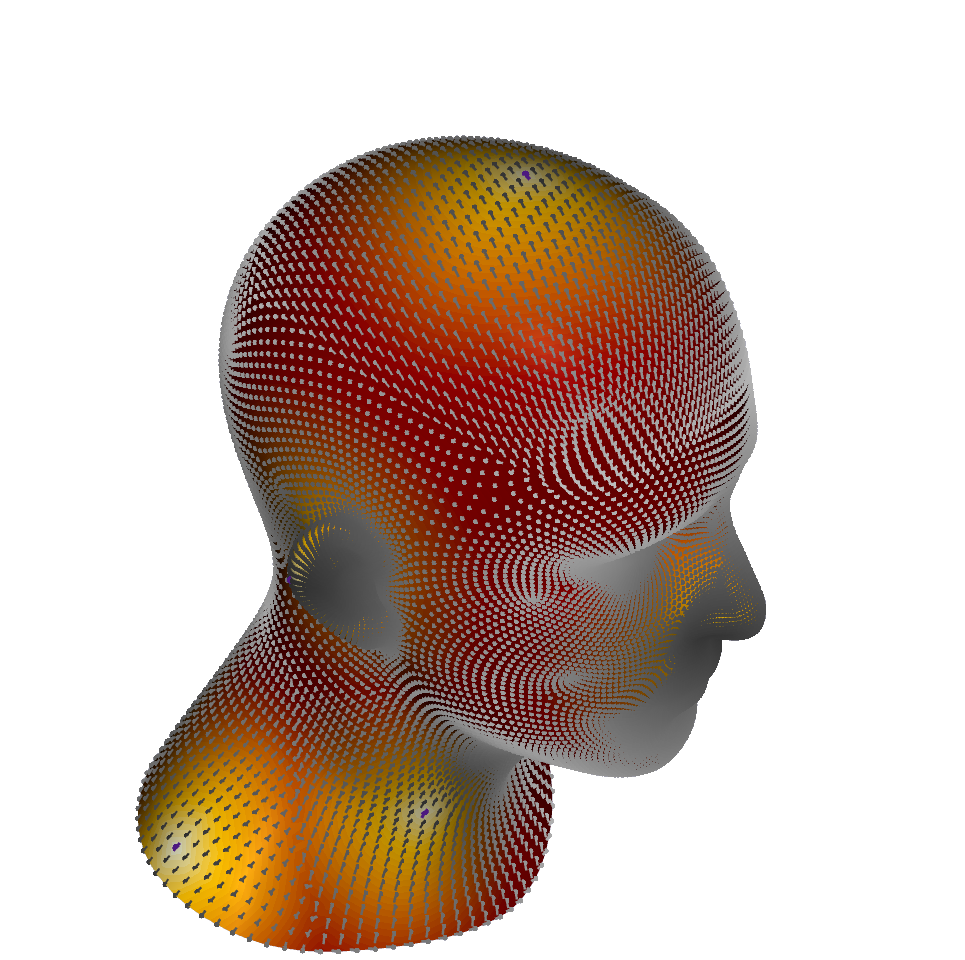
\includegraphics[width=7cm]{face_delaunay.png}
		\caption{Champs de vecteurs obtenus par transport optimal de plusieurs sources. A gauche la triangulation du maillage a été utilisée, à droite on utilise la triangulation de Delaunay. On remarque un vecteur ayant une norme très grande dans l'image de gauche et qui est corrigé par la triangulation de Delaunay à droite.}
		\label{fig:norme_delaunay}
	\end{figure}

	\paragraph{Autres discrétisations}
	Dans une section de l'article d'autres schémas de discrétisation sont donnés pour des types de données différentes : champs de 1-formes et $n$-champs. Il est aussi expliqué que pour d'autres représentations d'une variété pour lesquels on possède une discrétisation du Laplacien $L$, le Laplacien de connexion $L^\nabla$ peut être construit en utilisant le même procédé que précédemment, simplement en multipliant les coefficients qui ne sont pas sur la diagonale par les valeurs $r_{ij}$ de changement de face.
	
	\subsection{Propriétés et Résultats}
	
	La méthode de discrétisation proposée a le grand avantage de conserver plusieurs propriétés essentielles du transport parallèle quand on utilise une unique source :
	\begin{itemize}
		\item La méthode est linéaire : $P_\gamma \left( a X + Y \right) = a P_\gamma(X) + P_\gamma(Y)$.
		\item La norme est conservée : $| P_\gamma(X) | = | X |$.
		\item Une rotation du vecteur initial $X$ tourne le champ obtenu du même angle.
		\item La méthode est symétrique : $P_{\gamma_{y \rightarrow x}} \circ P_{\gamma_{x \rightarrow y}} = \text{id}$. Cela vient du fait que $L^\nabla$ soit Hermitienne.
	\end{itemize}
	
	\paragraph{Convergence}
	En notant $h$ la longueur moyenne des arrêtes du maillage, la méthode proposée semble converger en $\mathcal{O}(h)$, ce qui est moins bien que la méthode exacte traçant les géodésiques sur un polyèdre et qui possède une convergence quadratique $\mathcal{O}(h^2)$. Je n'ai pas testé cette convergence mais le papier montre un exemple de convergence sur un tore dont ils raffinent le maillage. La solution exacte étant facilement calculable théoriquement dans le cas d'un tore. Mais bien sûr les temps de calcul ne sont pas comparables, et l'avantage de la méthode présentée, est sa rapidité bien supérieur. Enfin comme pour le calcul des distances géodésiques, les meilleurs résultats sont obtenus en prenant $t = h^2$.
	
	\subsection{Applications}
	
	\paragraph{Extrapolation de vitesses}
	Finalement le papier propose plusieurs applications. La première est la possibilité d'extrapoler un champ de vitesses via le transport parallèle. Cette extrapolation peut s'avérer utile pour la composante normale de la vitesse dans la méthode des courbes de niveau. En cours nous avions surtout vu cette méthode dans des espaces euclidiens. Ici le papier donne la possibilité de l'étendre aux maillages.
	
	\paragraph{Calcul du log riemannien}
	La seconde application est la possibilité de calculer le log riemannien. Ce calcul est divisé en deux tâches. Le calcul de l'orientation et de la norme du logarithme. Pour cela on passe en coordonnées polaires :
	$$ \log_x(y) = r e^{\iota \varphi} $$
	Où $\varphi$ est l'angle dans la base locale du sommet $x$. On note $H_0=1$ le vecteur unitaire d'angle 0 dans cette base et $H = P_{\gamma_{x \rightarrow y}}(H_0)$ le champ obtenu par transport parallèle de ce vecteur. Puis pour $\epsilon$ suffisamment petit, on considère le cercle $C_\epsilon$ centré en $x$ et de rayon $\epsilon$ sur le plan tangent en $x$. On considère ensuite $\vec{n}(z)$, la normale de ce cercle orienté vers l'extérieur au point $z$. Ce cercle nous permet d'obtenir $\varphi$ via la formule suivante :
	$$ \varphi = \arg \left( P_{\gamma_{C_\epsilon \rightarrow y}}(\vec{n}) \right) - \arg \left( P_{\gamma_{x \rightarrow y}}(H_0) \right) = \arg R(y) - \arg H(y) $$
	Où $R = P_{\gamma_{C_\epsilon \rightarrow y}}(n)$ est le champ obtenu par transport parallèle de $\vec{n}$. La discrétisation de ce cercle et de sa normale $n$ est donnée en annexe du papier. On peut alors obtenir $\varphi$ en appliquant deux fois l'algorithme \ref{alg:VHM}. Quant-à $r$ il s'agit de la distance géodésique. On peut utiliser toute méthode déjà existante pour la calculer, dont la diffusion de la chaleur \cite{HM}. Mais le papier propose de réutiliser $R$ afin de factoriser les calculs. En effet $r$ peut être calculé à l'aide d'une simple équation de Poisson à partir de $R$. On a :
	$$ \Delta r = \nabla \cdot R $$
	\begin{center}
		\begin{tikzpicture}[scale=1.3]
			\coordinate (i) at (0, 0);
			\coordinate (j0) at ({1.3*cos(47)}, {-1.3*sin(47)});
			\coordinate (j1) at (1.5, 0);
			\coordinate (j2) at (0.9, 1.05);
			\coordinate (j3) at (-0.8, 1.05);
			\coordinate (j4) at (-1.4, 0.1);
			\coordinate (j5) at (-0.9, -0.95);
			
			\draw[thick] (i) -- (j0) -- (j1) -- (i) -- (j2) -- (j3) -- (i) -- (j4) -- (j5) -- (i);
			\draw[thick] (j1) -- (j2);
			\draw[thick] (j3) -- (j4);
			\draw[thick] (j5) -- (j0);
			
			\node[above=1pt] at (i) {$x$};
			\node[below=3pt, blue] at (i) {$C_\epsilon$};
			\node at (i) {$\bullet$};
			\node at (j0) {$\bullet$};
			\node at (j1) {$\bullet$};
			\node at (j2) {$\bullet$};
			\node at (j3) {$\bullet$};
			\node at (j4) {$\bullet$};
			\node at (j5) {$\bullet$};
			\draw[blue, thick] (i) circle(0.5);
			\foreach \i in {0,30,...,330}
				\draw[red, thick, ->] ({0.5*cos(\i)}, {0.5*sin(\i)}) -- ({0.84*cos(\i)}, {0.84*sin(\i)});
			\node[red] at (0.9, 0.45) {$\vec{n}$};
		\end{tikzpicture}
	\end{center}
	
	\begin{algorithm}[h]
		\caption{Log riemannien}
		\label{alg:log}
		\begin{algorithmic}
			\State \textbf{Entrée:} Un point $x$ d'une variété $M$.
			\State \textbf{Sortie:} La carte du logarithme en $x$ : $L(y) = r e^{\iota \varphi}$.
			\State \hspace{10pt} I. \; Transporter $H_0=1$ depuis $x$ sur tout $M$ via l'algorithme \ref{alg:VHM} pour obtenir $H$.
			\State \hspace{6pt} II. \; Transporter $\vec{n}$ depuis $C_\epsilon$ sur tout $M$ via l'algorithme \ref{alg:VHM} pour obtenir $R$.
			\State \, III. \; Calculer l'angle $\varphi = \arg R - \arg H$ à l'aide des deux champs précédents.
			\State \hspace{3pt} IV. \; Calculer la norme $r$ via l'équation de Poisson : $ \Delta r = \nabla \cdot R$.
		\end{algorithmic}
	\end{algorithm}
	Un exemple de carte logarithme est donné \figurename~\ref{fig:bimba}. Encore une fois le résultat est fortement impacté par la qualité du maillage. Un cas extrême est donné \figurename~\ref{fig:car} sur un sommet dont les faces auxquels il appartient sont très allongés. Cela donne une forte anisotropie dans la distance $r$ et l'orientation est assez chaotique. Sur la \figurename~\ref{fig:log_bunny}, un autre type de difficulté est mis en évidence, le cas où la quasi totalité de la surface est accessible en partant dans une direction quasi identique.
	
	\begin{figure}
		\centering
		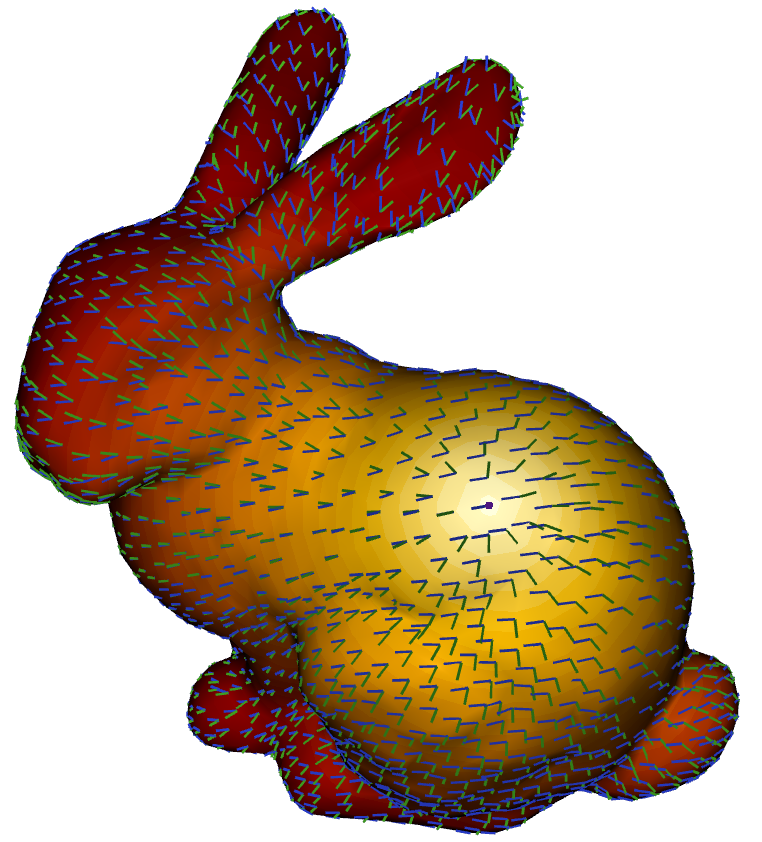
\includegraphics[width=7cm]{log1_bunny.png} \; 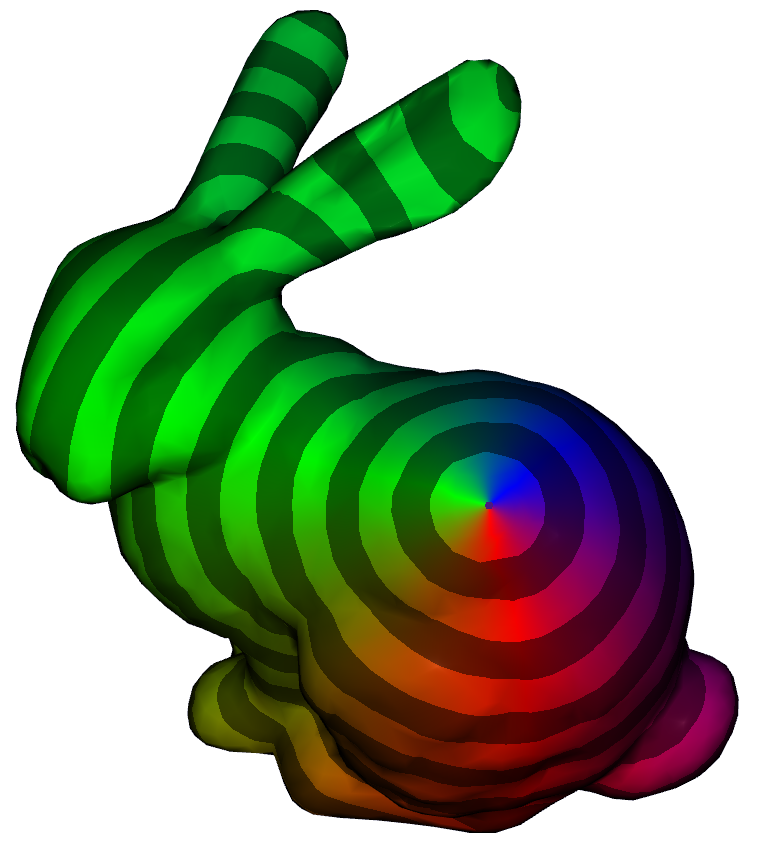
\includegraphics[width=7cm]{log2_bunny.png}
		\caption{Carte logarithme sur le maillage \texttt{bunny.obj}. A gauche les deux champ $H$ (en bleu) et $R$ (en vert) sont représentés. A droite se trouve une représentation de la carte. La couleur indique l'orientation en utilisant le disque RGB où le rouge représente l'angle 0, le bleu l'angle $2\pi/3$ et le vert l'angle $4\pi/3$. Les bandes claires/foncées sont des lignes d'équidistances.}
		\label{fig:HR}
	\end{figure}

	\begin{figure}
		\centering
		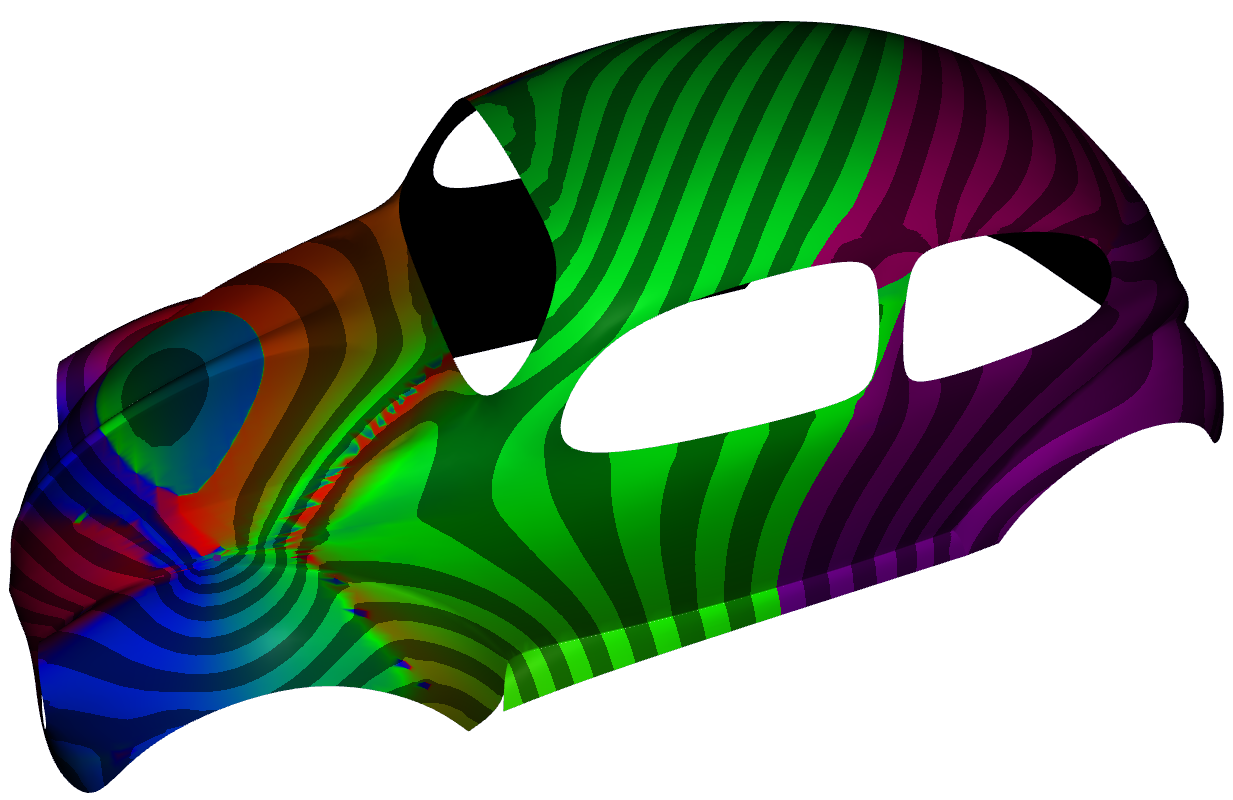
\includegraphics[width=7.5cm]{log_car_without_d.png} \; 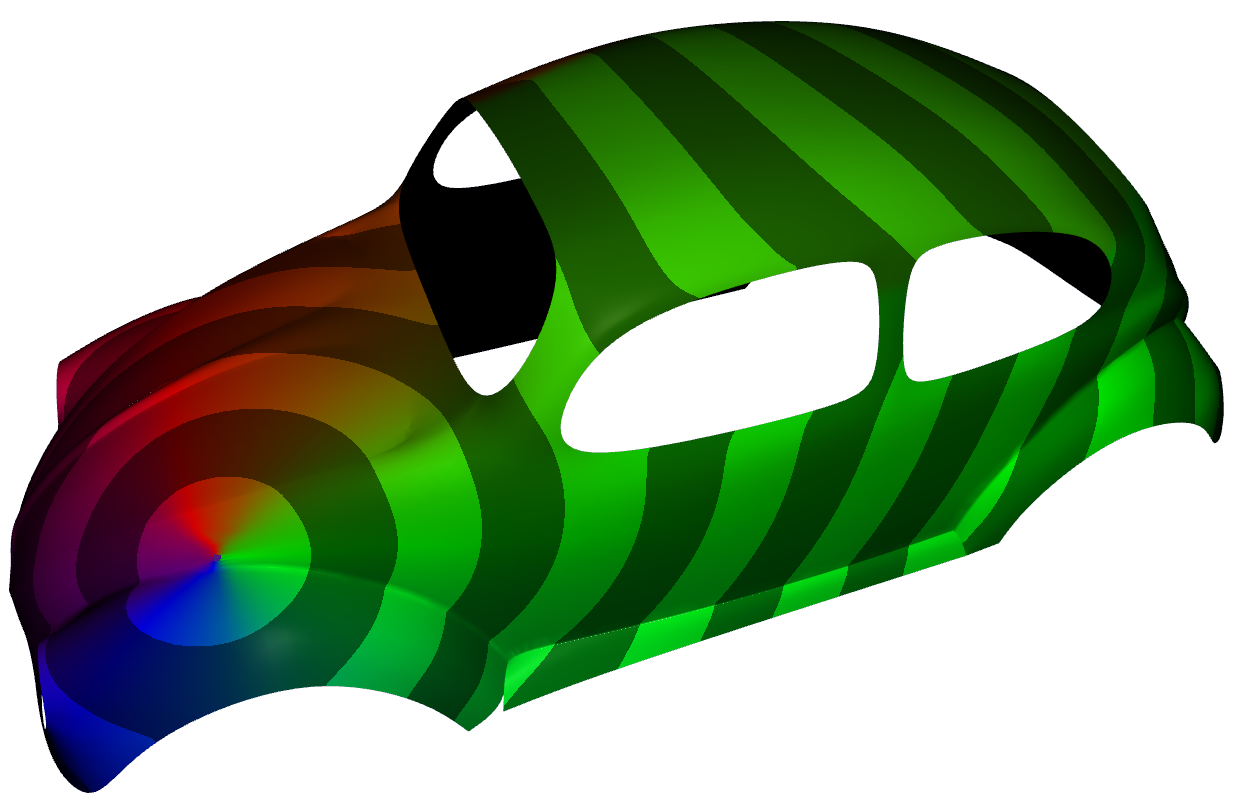
\includegraphics[width=7.5cm]{log_car_with_d.png}
		\caption{Carte logarithme sur le maillage \texttt{beetle.off}. A gauche la triangulation du maillage a été utilisée, à droite on utilise la triangulation de Delaunay. On remarque une importante différence de qualité. L'image de gauche est même complètement fausse.}
		\label{fig:car}
	\end{figure}

	\paragraph{Moyenne de Karcher et médiane géométrique}
	
	La moyenne $\bar{x}$ de $n$ points $y_1, ..., y_n$ dans les espaces euclidiens peut être généralisée aux variétés par les minimiseurs de l'énergie de Fréchet $E$ définie par :
	$$ E_p(x) = \frac{1}{2n} \sum_{i=1}^n d(x, y_i)^p $$
	Où $d$ est une distance sur l'espace. Dans le cas des variétés/maillage, il s'agit de la distance géodésique. Pour $p=2$ on appelle moyenne de Karcher les minimiseurs de cette énergie (s'il y a unicité on parle aussi de moyenne de Fréchet) et pour $p=1$, on parle de médiane géométrique. Dans ce cas $p = 1$, le résultat obtenu est plus robuste face aux valeurs aberrantes. Jusqu'à cet article on ne savait pas vraiment calculer une telle moyenne. Mais on peut remarquer que le gradient de $E$ s'exprime en fonction du logarithme en $x$ :
	$$ \nabla E_p = - \frac{p}{2n} \sum_{i=1}^n \log_x(y_i) d(x, y_i)^{p-2} $$
	On peut alors calculer des moyennes en utilisant une descente de gradient qui ne nécessite qu'un calcul de carte logarithme en $x$ à chaque étape. Comme on calcule la carte logarithme en entier, le nombre $n$ de points n'impacte pas le temps de calcul. On peut d'ailleurs tout à fait calculer une moyenne/espérance d'une distribution $\rho$ sur $M$. Ainsi le cas des $n$ points est obtenus avec $\rho = \frac{1}{n} \sum_{i=1}^n \delta_{y_i}$. Voici un algorithme dans le cas général des distribution :
	\begin{algorithm}[h]
		\caption{$p$-Moyenne}
		\label{alg:moy}
		\begin{algorithmic}
			\State \textbf{Entrée:} Une distribution $\rho$ sur $M$ [et $\tau$ un pas de déplacement].
			\State \textbf{Sortie:} Un sommet $x$ minimisant l'énergie $E_p$.
			\State \hspace{7pt} I. \; Choisir $x_0 \in M$ aléatoirement.
			\State \hspace{3pt} II. \; Jusqu'à ce que la norme de $v$ soit suffisamment petite :
			\State \hspace{16pt} (a) \, Calculer la carte logarithme $\log_{x_k} = r e^{\iota \varphi}$ via l'algorithme \ref{alg:log}.
			\State \hspace{16pt} (b) \, Calculer la direction du gradient $v = \sum_{y \in M} \rho(y) \log_{x_k}(y) r(y)^{p-2}$.
			\State \hspace{16pt} (c) \, Mettre à jour $x$ via $x_{k+1} = x_k + \exp_{x_k}(\tau v)$.
		\end{algorithmic}
	\end{algorithm}

	\paragraph{Tesselations de Voronoï centrées}
	La possibilité de calculer la moyenne d'une distribution sur $M$ permet de pouvoir effectuer une relaxation de LLoyd sur un diagramme de Voronoï afin de calculer une tesselation de Voronoï centrée. Pour un ensemble de sites $s_i$, on peut approximer les cellules de Voronoï par les distributions :
	$$ \rho_i = \frac{k_t(s_i, \cdot)}{\sum_j k_t(s_j, \cdot)} \qquad \text{au lieu de} \qquad \rho_i(x) = \mathbbm{1} \left\{ i = \argmin_j d(s_j, x) \right\} $$
	Puis la mise à jour des centres se fait via une étape du calcul de la moyenne des distributions $\rho_i$. Cela nous donne l'algorithme \ref{alg:TVC}.
	\begin{algorithm}[h]
		\caption{Tesselation de Voronoï centrée}
		\label{alg:TVC}
		\begin{algorithmic}
			\State \textbf{Entrée:} Un ensemble de sites initiaux $s_i$ sur $M$.
			\State \textbf{Sortie:} Les sites $s_i$ sont désormais les centres de leurs cellules de Voronoï.
			\State \hspace{7pt} I. \; Jusqu'à convergence des sites $s_i$ :
			\State \hspace{10pt} (a) \, Calculer les densités $\rho_i = k_t(s_i, \cdot) / \sum_j k_t(s_j, \cdot)$.
			\State \hspace{10pt} (b) \, Appliquer une étape de l'algorithme \ref{alg:moy} pour chaque $s_i$ avec la distribution $\rho_i$.
		\end{algorithmic}
	\end{algorithm}
	
	\paragraph{\textit{Landmarks} ordonnés}
	Enfin la dernière application proposée est le calcul de \textit{landmarks} ordonnés sur un ensemble de surfaces légèrement déformées afin de pouvoir effectuer certaines correspondances. L'idée est de calculer une médiane  géométrique sur la surface via l'algorithme \ref{alg:moy} (en prenant une distribution uniforme sur la surface) puis d'utiliser un échantillonnage des points les plus loin pour construire nos \textit{landmarks}. Pour plus de stabilité, l'algorithme propose de calculer plusieurs médianes puis de commencer l'échantillonnage en ne prenant aucune des médianes dans l'ensemble de \textit{landmarks}.
	
	\section{Implémentation}
	
	Nicholas Sharp développe sa propre librairie de géométrie en C++ nommée geometry central (\url{https://geometry-central.net/}). Les codes disponibles pour ce papier sont alors implémenté dans cette librairie que j'avais d'ailleurs utilisée durant mon stage de L3. En me renseignant j'ai découvert une autre librairie de géométrie qui semble bien plus utilisée que geométry central. C'est librairie est \verb|libigl| (\url{https://libigl.github.io/}). J'ai donc décidé de prendre en main cette libraire et d'y implémenter le transport parallèle proposé par l'article, ainsi que le calcul du logarithme riemannien. Le code est très rapide. Tout se fait en une fraction de seconde. Il est aussi possible de switcher entre la triangulation du maillage et la triangulation de Delaunay pour comparer. Les images dans ce rendu ont été faites avec mon code. Je vais continuer de bosser dessus en faisant notamment les autres applications et j'essaierai de faire rentrer mon implémentation dans la librairie. Voici l'adresse de mon repo github : \url{https://github.com/Nanored4498/Vector-Heat-Method}.
	
	\begin{figure}
		\centering
		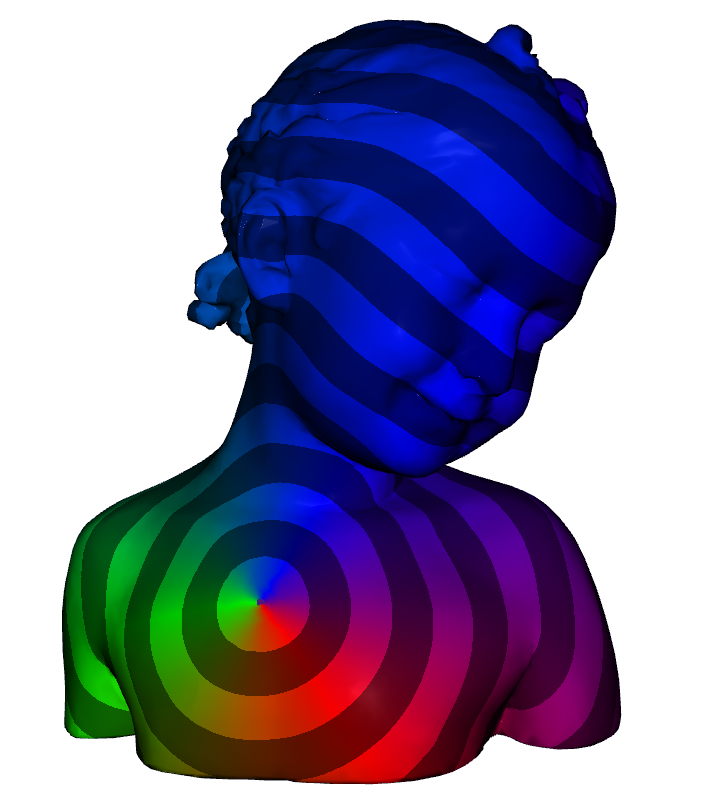
\includegraphics[width=7cm]{bimba_log.png}
		\caption{Carte logarithme sur le maillage \texttt{bimba.obj}. La couleur indique l'orientation en utilisant le disque RGB où le rouge représente l'angle 0, le bleu l'angle $2\pi/3$ et le vert l'angle $4\pi/3$. Les bandes claires/foncées sont des lignes d'équidistances.}
		\label{fig:bimba}
	\end{figure}

	\begin{figure}
		\centering
		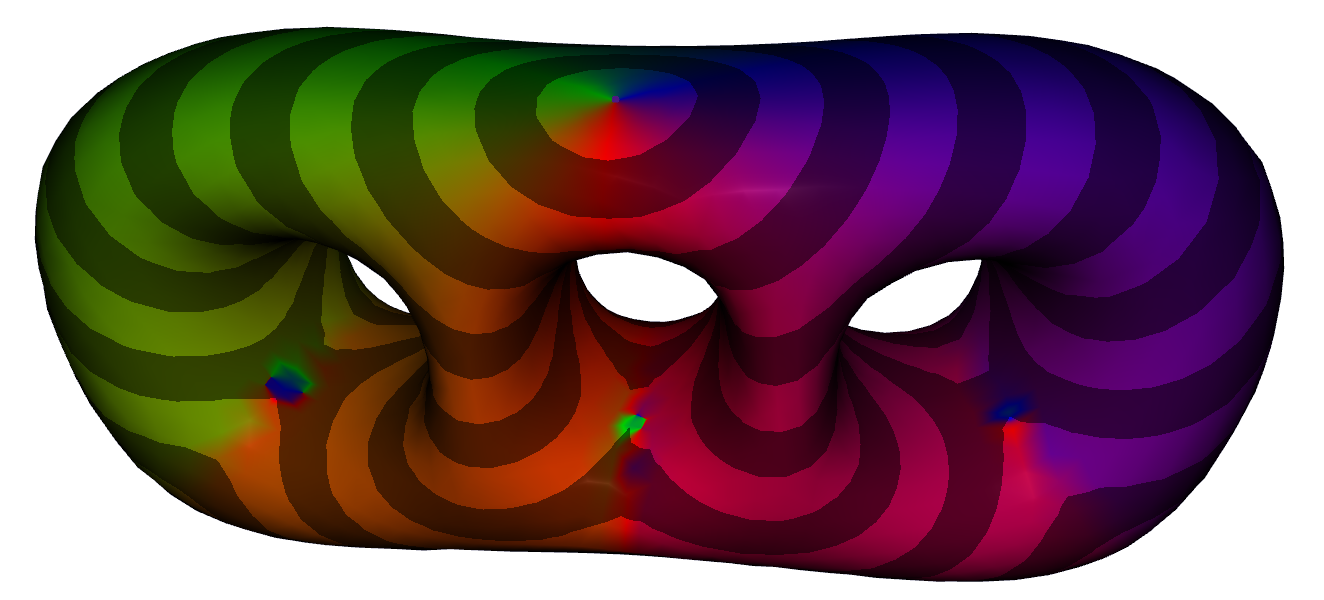
\includegraphics[width=14cm]{log_cut_locus.png}
		\caption{Carte logarithme sur le maillage \texttt{3holes.off}. On peut remarquer des petites erreurs de calculs au niveau des coutures (en bas des trois trous), c'est à dire au niveau des sommets qui ont plusieurs plus courts chemins possibles à la source.}
		\label{fig:cut_locus}
	\end{figure}

	\begin{figure}
		\centering
		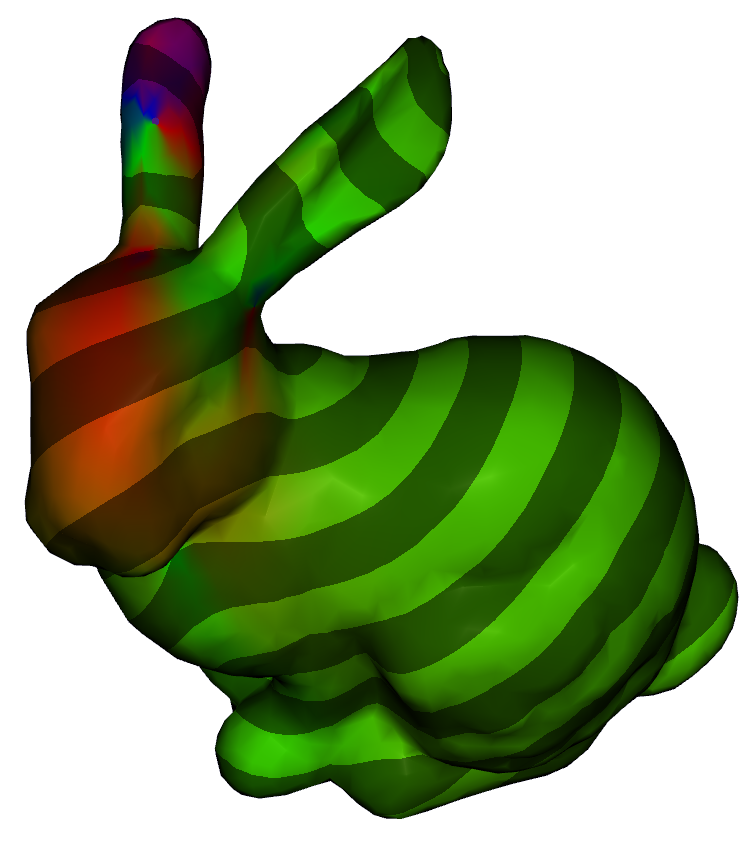
\includegraphics[width=7.5cm]{log_without_delaunay.png} \; 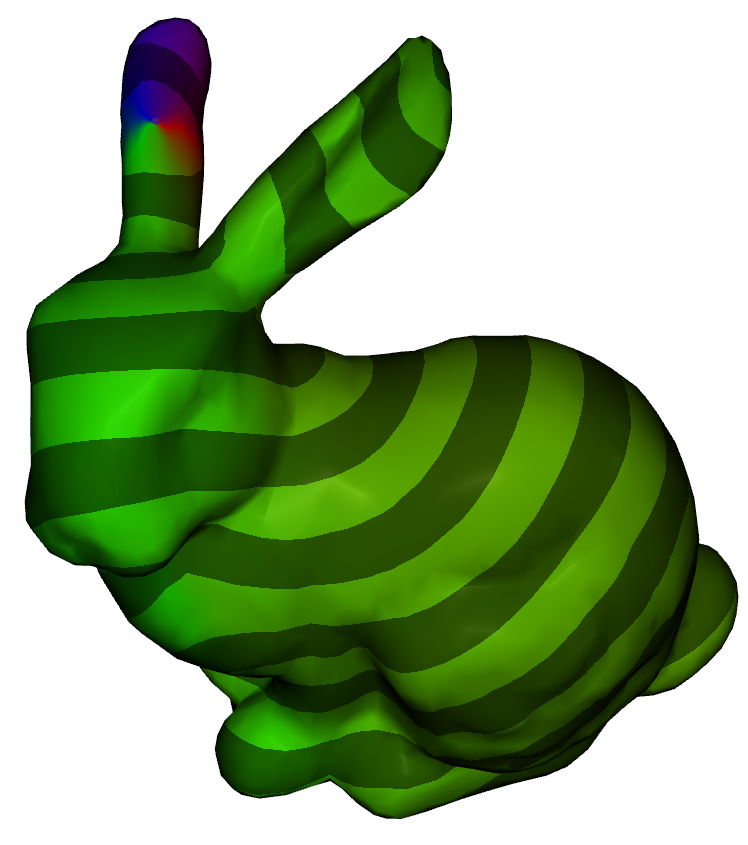
\includegraphics[width=7.5cm]{log_with_delaunay.png}
		\caption{Carte logarithme sur le maillage \texttt{bunny.obj}. A gauche la triangulation du maillage a été utilisée, à droite on utilise la triangulation de Delaunay. La source est choisi sur une oreille qui est une condition un peu extrême car une grande partie de la surface est accessible en partant dans une direction similaire (d'où le fait que le lapin soit presque entièrement vert). Sans la triangulation de Delaunay l'algorithme commet des erreurs visibles sur la tête du lapin.}
		\label{fig:log_bunny}
	\end{figure}

	\appendix
	
	\bibliographystyle{alpha}
	\bibliography{bib.bib}

\end{document}